\documentclass[11pt]{article}
\usepackage[utf8]{inputenc}
\usepackage[margin=1in]{geometry}
\usepackage{amsmath,amssymb}
\usepackage{graphicx}
\usepackage{booktabs}
\usepackage{float}
\usepackage{setspace}
\usepackage[round]{natbib}
\usepackage[hidelinks]{hyperref}
\onehalfspacing

\title{Concentrated Sectors Transmit Less:\\Within-Sector Concentration and Time-Varying Connectedness\\in the S\&P 500, 2018 to 2026}
\author{Tanishk Yadav\thanks{Department of Finance and Risk Engineering, New York University Tandon School of Engineering, New York, NY, USA. Email: \texttt{ty2766@nyu.edu}.}}
\date{September 2026}

\begin{document}
\maketitle

\begin{abstract}
\noindent
The ten largest firms rose from 24\% to 41\% of S\&P 500 market capitalization between 2018 and 2025. This paper asks what that concentration did to the way shocks travel between the eleven GICS sectors. Using daily returns and range-based volatilities of the Select Sector SPDR funds from October 2018 to August 2026, a point-in-time constituent panel with historical share counts, and a filtered TVP-VAR connectedness model, I report three results. First, sector connectedness is contemporaneous rather than lead-lag. Classical Granger F-tests appear to find 90 of 110 significant directed links after false-discovery-rate control, but the classical test rejects 21 to 31\% of the time at a nominal 5\% under GARCH errors, and heteroskedasticity-robust tests leave no significant link, in the full sample or either half. The classical rejections come almost entirely from February to June 2020, a market-wide daily reversal rather than sector-to-sector transmission, and lagged cross-sector returns have negative out-of-sample $R^2$ for all eleven sectors. Second, total connectedness peaked at 88.9\% on 16 March 2020 and fell to 53.7\% in August 2026, its lowest level in the sample, while index concentration reached records; a 200-day rolling window understates the April 2025 tariff shock and then records a spurious drop of more than 20 points when the shock leaves the window. Third, with sector and month fixed effects, a sector whose three largest firms gain market share transmits fewer shocks to the other sectors: one percentage point of top-three share lowers net directional connectedness by 0.47 points ($t=-3.6$), and by 0.66 points ($t=-4.8$) when returns and concentration share the same uncapped weights. Concentrated sectors also co-move less with the rest of the market, consistent with firm-level (granular) shocks dominating their returns.

\medskip
\noindent\textbf{Keywords:} connectedness, TVP-VAR, generalized variance decomposition, market concentration, granularity, Granger causality, heteroskedasticity-robust inference, sector returns
\\\noindent\textbf{JEL:} C32, C58, G11, G12, L11
\end{abstract}

\newpage
%============================================================
\section{Introduction}
%============================================================

U.S. equity market concentration is at its highest level in decades. In our constituent panel the ten largest firms held 24\% of S\&P 500 market capitalization at the end of 2018 and 41\% at the end of 2025. Concentration is not only an index-level fact. Within sectors it is higher still: by August 2026 the three largest firms held 82\% of Communication Services and 54\% of Information Technology, against 18\% of Industrials.

A large literature measures how shocks propagate across sectors, industries, and asset classes through the connectedness framework of \citet{diebold2009, diebold2012, diebold2014}. A separate literature, following \citet{gabaix2011}, argues that when a few firms are large relative to their aggregate, firm-specific shocks no longer diversify away and become aggregate shocks. The two literatures have not met. If a sector's return is increasingly driven by the news of two or three firms, that sector's shocks should look less like common sector news and more like idiosyncratic noise from the point of view of other sectors. Concentration should then change a sector's role in the connectedness network.

This paper tests that prediction on the eleven GICS sectors of the S\&P 500 from October 2018 to August 2026, a window that contains the late-2018 sell-off, the COVID-19 crash, the 2022 rate shock, the March 2023 regional bank failures, and the April 2025 tariff shock. Three design choices matter. Sector returns come from the Select Sector SPDR funds, which track the full GICS sectors with point-in-time membership, rather than from today's constituents. Concentration comes from a separate constituent panel that uses point-in-time index membership, historical share counts, and the March 2023 GICS reclassification. Time variation comes from a TVP-VAR estimated by a forgetting-factor Kalman filter \citep{koop2013, antonakakis2020}, so each daily estimate uses only data available that day.

The paper makes three contributions.

The first is a correction to a common inference. Daily sector returns carry strong conditional heteroskedasticity, and pairwise Granger tests on them are widely reported with classical F statistics. On our data the classical test, with the minimum $p$-value taken over lags one to five, finds 90 of 110 directed links significant after Benjamini-Hochberg control. A Monte Carlo calibrated to the same data, with GARCH(1,1)-$t$ dynamics, a common factor, and no lead-lag by construction, shows that this test rejects 31\% of the time at a nominal 5\%. Heteroskedasticity-robust Wald tests are correctly sized, and with them no directed link survives multiplicity control in the full sample, in either half, or within 2020. The classical rejections are concentrated in February to June 2020, 4.6\% of trading days that carry 97.6\% of the lagged cross-sector covariance; in that window every sector's lagged return predicts every other sector's with about the same negative coefficient as its own, the signature of a market-wide daily reversal. Out of sample, lagged cross-sector returns do not beat the historical mean for any sector. Sector connectedness is contemporaneous.

The second contribution is a filtered, daily history of return and volatility connectedness through August 2026. Total return connectedness peaked at 88.9\% on 16 March 2020 and reached its sample low of 53.7\% in late August 2026. Volatility connectedness shows the same shape. A 200-day rolling window, the default in applied work, understates the April 2025 jump and then drops by more than 20 points 200 trading days later, when the shock leaves the window. The filtered estimates show neither artifact.

The third contribution is the link between concentration and connectedness. In a monthly sector panel with sector and month fixed effects and Driscoll-Kraay standard errors, a one-percentage-point rise in a sector's top-three share lowers its net directional connectedness by 0.47 points and the connectedness it transmits by 0.50 points, while what it receives does not change significantly. When returns are rebuilt from constituents with the same uncapped weights used to measure concentration, the effects rise to 0.66 and 0.83 points, and the Herfindahl index becomes significant as well. The results hold without Information Technology and Communication Services, the two sectors most affected by fund-level weight caps. A direct test supports the granular interpretation: concentrated sectors have a lower monthly $R^2$ against the rest of the market. The relationship is a level relationship; it is not detectable in month-to-month changes, which is expected when concentration moves slowly.

The rest of the paper is organized as follows. Section~\ref{sec:lit} places the paper in the literature. Section~\ref{sec:data} describes the data. Section~\ref{sec:method} sets out the econometrics. Section~\ref{sec:results} reports results, and Section~\ref{sec:disc} discusses them.

%============================================================
\section{Related literature}\label{sec:lit}
%============================================================

\textbf{Connectedness.} \citet{diebold2009} measure spillovers with forecast-error variance decompositions from a VAR; \citet{diebold2012} replace the Cholesky decomposition with the order-invariant generalized decomposition of \citet{koop1996} and \citet{pesaran1998}, which also yields directional measures; \citet{diebold2014} link the measures to network degree. Time variation was first estimated with rolling windows, whose length is arbitrary and whose estimates react to a shock twice, on entry and on exit. \citet{antonakakis2020} replace the window with a TVP-VAR estimated by the forgetting-factor Kalman filter of \citet{koop2013}, and \citet{barunik2018} decompose connectedness by frequency. \citet{billio2012} measure system-wide linkages among financial institutions with principal components and Granger networks.

\textbf{Cross-industry predictability.} A lead-lag literature argues that information diffuses slowly across economically linked industries: \citet{hou2007} finds that large firms lead small firms within industries, \citet{menzly2010} document cross-predictability along supply chains at monthly frequency, and \citet{hong2007} report that some industries lead the aggregate market. \citet{rapach2019} find out-of-sample industry predictability at monthly frequency using regularized regressions. The present paper asks the daily question for broad sectors and applies the out-of-sample criteria of \citet{campbell2008} and \citet{clark2007}.

\textbf{Concentration and granularity.} \citet{gabaix2011} shows that when the firm-size distribution is fat-tailed, idiosyncratic shocks to large firms generate aggregate fluctuations. \citet{grullon2019} document rising concentration across U.S. industries. \citet{campbell2001} show that idiosyncratic volatility is a large and time-varying part of stock risk, and \citet{pollet2010} relate average correlation to future market returns. To our knowledge, no study relates within-sector concentration to a sector's position in the connectedness network.

%============================================================
\section{Data}\label{sec:data}
%============================================================

\subsection{Sector returns and volatility}

Sector returns are daily log returns, in percent, of the eleven Select Sector SPDR funds (XLC, XLY, XLP, XLE, XLF, XLV, XLI, XLK, XLB, XLRE, XLU), adjusted for distributions. The sample runs from 1 October 2018 to 31 August 2026, 1,989 trading days. The start date follows the September 2018 GICS reorganization that created Communication Services. The funds have three advantages over sector returns built from today's constituents: they cover every member of each sector, their membership is point-in-time, and they are investable. Their disadvantage is weight capping, which limits single-name weights and therefore understates concentration where it is highest. We address this with a second return series built from constituents without caps (Section~\ref{sec:const}).

Volatility is the \citet{parkinson1980} range estimator, $\hat\sigma^2_t = (\ln H_t - \ln L_t)^2/(4\ln 2)$, annualized and in logs, $v_t = \ln(100\sqrt{252\,\hat\sigma^2_t})$. Table~\ref{tab:desc} reports summary statistics. Every sector has negative skewness and excess kurtosis between 7 and 17. Log volatility is persistent, with first-order autocorrelation between 0.50 and 0.63.

\subsection{Constituents, market capitalization, and concentration}\label{sec:const}

Concentration is measured from individual firms. Index membership is point-in-time: current members enter on their S\&P 500 addition date, and firms removed during the sample enter and leave on their actual dates. Removed firms are kept when price and share data remain available, which recovers 78 firms; firms that were acquired and delisted cannot be recovered. A removed ticker whose price path duplicates a current ticker is treated as a rename rather than a second firm. The resulting panel covers 428 firms on the first day and 497 on the last.

Market capitalization is the daily closing price times historical shares outstanding, with both series on the same split basis and a five-day rolling median applied to the vendor share series to remove recording spikes. Using historical rather than current share counts matters for firms with large buybacks or issuance over the sample. Firms with two listed share classes are counted once, because the vendor reports firm-level shares on both lines. Firms are assigned to GICS sectors with the March 2023 reclassification applied on its effective date: payment processors are in Information Technology before 17 March 2023 and in Financials after, and Target, Dollar General, and Dollar Tree move from Consumer Discretionary to Consumer Staples on the same date.

For sector $s$ on day $t$, with market-capitalization weights $w_{i,t}$ inside the sector, the two concentration measures are the Herfindahl index $\text{HHI}_{s,t} = \sum_i w_{i,t}^2$ and the top-three share, the sum of the three largest weights. Both use total rather than float-adjusted market capitalization, which is the economically relevant size for the granular argument and differs from index weights for firms with large insider holdings. The index-level top-ten share computed this way is 24.1\% at the end of 2018, 33.0\% at the end of 2023, and 40.8\% at the end of 2025, within one to three points of published float-adjusted figures.

Figure~\ref{fig:conc} shows the top-three share by sector. Concentration rose most in Communication Services (62\% to 82\%), Consumer Discretionary (48\% to 65\%), Information Technology (45\% to 55\%), and Consumer Staples (38\% to 49\%), and fell slightly in Industrials, Financials, and Energy.

A second, uncapped return series weights each constituent's daily return by its previous-day market capitalization inside its sector. Its daily correlation with the corresponding fund is between 0.986 and 0.999 for ten sectors and 0.926 for Communication Services, where fund caps bind hardest.

\begin{table}[H]
\centering
\caption{Summary statistics, 1 October 2018 to 31 August 2026 (1,989 days)}
\label{tab:desc}
\small
\begin{tabular}{lrrrrrrrr}
\toprule
& \multicolumn{4}{c}{Daily log return} & \multicolumn{2}{c}{Log range volatility} & \multicolumn{2}{c}{Top-3 share (\%)} \\
\cmidrule(lr){2-5}\cmidrule(lr){6-7}\cmidrule(lr){8-9}
Sector & Mean & Vol. & Skew & Ex. kurt. & Mean & AR(1) & 2018Q4 & 2026 \\
\midrule
Communication Services & 11.4 & 22.4 & $-0.47$ & 7.1 & 2.54 & 0.57 & 62.1 & 82.3 \\
Consumer Discretionary & 9.6 & 24.3 & $-0.51$ & 7.3 & 2.61 & 0.63 & 47.7 & 65.4 \\
Consumer Staples & 8.4 & 15.8 & $-0.42$ & 14.3 & 2.29 & 0.53 & 38.3 & 49.2 \\
Energy & 11.0 & 32.4 & $-0.95$ & 14.9 & 2.92 & 0.58 & 54.7 & 54.0 \\
Financials & 11.2 & 23.6 & $-0.58$ & 15.5 & 2.53 & 0.58 & 35.8 & 31.0 \\
Health Care & 9.1 & 17.7 & $-0.33$ & 9.5 & 2.40 & 0.50 & 27.7 & 33.4 \\
Industrials & 11.8 & 21.6 & $-0.48$ & 12.6 & 2.49 & 0.58 & 19.4 & 17.9 \\
Information Technology & 21.2 & 27.2 & $-0.26$ & 7.5 & 2.69 & 0.55 & 44.7 & 54.8 \\
Materials & 9.6 & 22.2 & $-0.40$ & 9.3 & 2.55 & 0.55 & 36.6 & 36.9 \\
Real Estate & 7.1 & 22.2 & $-1.04$ & 17.4 & 2.59 & 0.51 & 27.5 & 32.0 \\
Utilities & 9.0 & 20.6 & $-0.25$ & 15.0 & 2.59 & 0.50 & 27.6 & 27.9 \\
\bottomrule
\end{tabular}

\smallskip
\parbox{0.95\textwidth}{\footnotesize Mean and volatility of returns are annualized, in percent. Log range volatility is the log of the annualized Parkinson volatility in percent. The top-three share is the average of daily values over October to December 2018 and over January to August 2026.}
\end{table}

\begin{figure}[H]
\centering
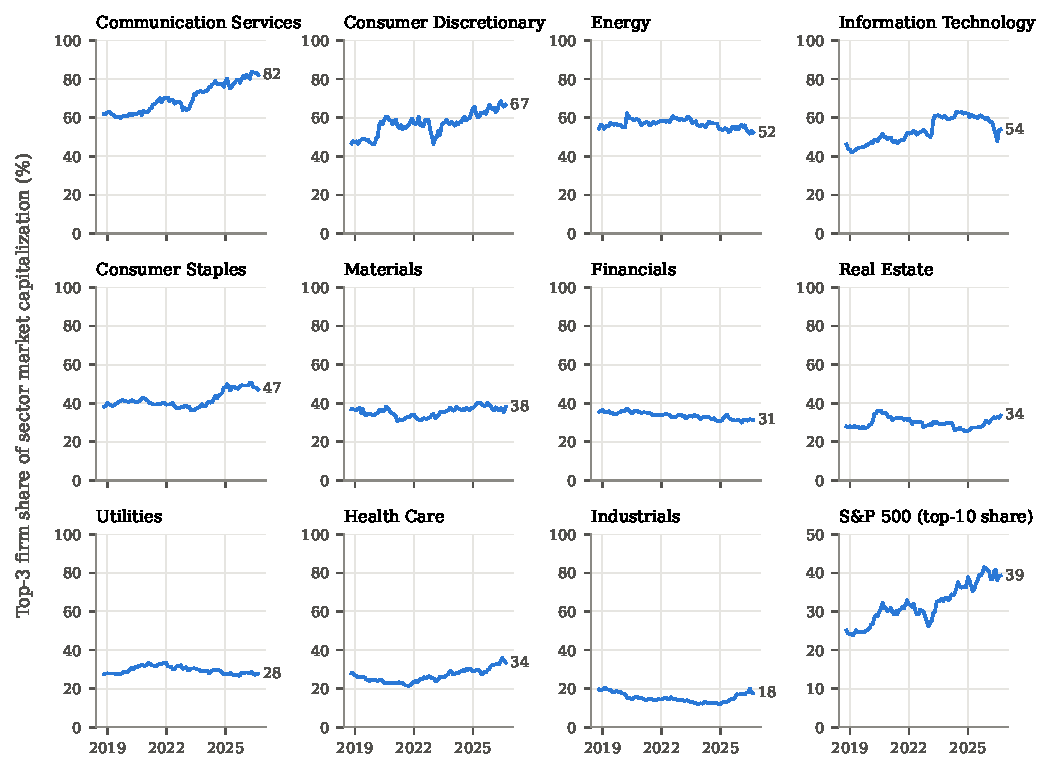
\includegraphics[width=\textwidth]{fig/fig3_concentration.pdf}
\caption{Share of sector market capitalization held by the three largest firms, month-end, October 2018 to August 2026. The last panel is the top-ten share of the whole index. Values at the right edge are August 2026.}
\label{fig:conc}
\end{figure}

%============================================================
\section{Methodology}\label{sec:method}
%============================================================

\subsection{Generalized connectedness}

Let $y_t$ be the $k=11$ vector of sector returns (or log volatilities), with VAR($p$) representation $y_t = c + \sum_{l=1}^{p} B_l y_{t-l} + u_t$, $u_t \sim (0,\Sigma)$, and moving-average coefficients $\Phi_h$. The generalized forecast-error variance decomposition of \citet{pesaran1998} at horizon $H$ is
\begin{equation}
\theta_{ij}(H) = \frac{\sigma_{jj}^{-1}\sum_{h=0}^{H-1}\left(e_i'\Phi_h\Sigma e_j\right)^2}{\sum_{h=0}^{H-1} e_i'\Phi_h\Sigma\Phi_h' e_i},
\qquad \tilde\theta_{ij}(H) = \frac{\theta_{ij}(H)}{\sum_{j}\theta_{ij}(H)},
\end{equation}
the share of sector $i$'s $H$-step forecast-error variance attributable to shocks in sector $j$. Following \citet{diebold2012}, in percent,
\begin{equation}
\text{FROM}_i = \sum_{j\neq i}\tilde\theta_{ij}, \quad \text{TO}_j = \sum_{i\neq j}\tilde\theta_{ij}, \quad \text{NET}_i = \text{TO}_i - \text{FROM}_i, \quad \text{TCI} = \frac{1}{k}\sum_{i\neq j}\tilde\theta_{ij}.
\end{equation}
We set $H=10$ and choose $p$ by BIC. For daily returns BIC selects no lags and we use $p=1$; for log volatility it selects $p=1$.

\subsection{Time-varying parameter VAR}

The TVP-VAR is $y_t = Z_t\beta_t + u_t$ with $Z_t = I_k\otimes(1, y_{t-1}')$, $\beta_t = \beta_{t-1}+\xi_t$, and $u_t\sim(0,\Sigma_t)$. Following \citet{koop2013} and \citet{antonakakis2020}, the state covariance is inflated by a forgetting factor rather than estimated, $P_{t|t-1} = P_{t-1|t-1}/\kappa_1$, and the measurement covariance is an exponentially weighted average of prediction errors, $\Sigma_t = \kappa_2\Sigma_{t-1}+(1-\kappa_2)\hat u_t\hat u_t'$, with $\kappa_1=\kappa_2=0.99$. The intercept is included because log volatility has a large mean. The filter starts on 20 June 2018 with $\beta_0=0$ and $P_0 = 0.1I$, and estimates before 1 October 2018 are discarded as burn-in. We use filtered, not smoothed, estimates, so the connectedness measure on day $t$ uses only data through day $t$. At each date the measures in (2) are computed from $(\beta_{t|t},\Sigma_t)$.

\subsection{Granger causality}

For each ordered pair $(j, i)$ we test whether lags of $y_j$ enter the equation for $y_i$. The system version conditions on the lags of all eleven sectors; the bivariate version conditions only on lags of $y_i$. Test statistics are Wald statistics with the HC3 covariance estimator, which is valid under conditional heteroskedasticity of unknown form. For comparison we also report classical F statistics. Across the 110 ordered pairs, $p$-values are adjusted with the \citet{benjamini1995} false-discovery-rate procedure and with Bonferroni.

\subsection{Out-of-sample predictability}

For each sector we forecast the next day's return from the current returns of all eleven sectors, re-estimating by OLS on an expanding window that starts with the first quarter of the sample, so the evaluation period begins on 23 September 2020. The unrestricted regression is noisy with eleven predictors, so we also report the equal-weighted combination of eleven single-predictor forecasts. The benchmark is the prevailing historical mean. We report $R^2_{OS} = 1 - \sum(r - \hat r)^2/\sum(r-\bar r)^2$ \citep{campbell2008} and the \citet{clark2007} test with Newey-West variance.

\subsection{Concentration and connectedness}

Daily TVP-VAR measures are averaged to months and merged with month-end concentration from the previous month. The baseline regression is
\begin{equation}
C_{s,m} = \alpha_s + \delta_m + \gamma\,\text{Conc}_{s,m-1} + \phi_1\ln(\text{share}_{s,m-1}) + \phi_2 \bar v_{s,m} + \varepsilon_{s,m},
\end{equation}
where $C$ is FROM, TO, or NET, Conc is the top-three share or the HHI (both in percentage points), share is the sector's weight in the index, and $\bar v$ is the sector's average log volatility in the month. Sector fixed effects remove permanent differences between sectors, and month fixed effects remove anything common to all sectors in a month, including the level of system connectedness and market volatility. Standard errors follow \citet{driscoll1998} with three lags, which allows cross-sectional dependence and serial correlation. The panel has 11 sectors and 94 months, November 2018 to August 2026.

%============================================================
\section{Results}\label{sec:results}
%============================================================

\subsection{Static connectedness}

Over the full sample the total connectedness index is 79.5\% for returns and 77.7\% for volatility (Table~\ref{tab:static}). Industrials is the largest net transmitter in both systems, followed by Materials and Financials for returns. Energy is the largest net receiver of return shocks and Utilities of volatility shocks.

The return index barely moves with the VAR specification: across lag orders 1, 2, and 5 and horizons 5, 10, and 20 it ranges from 79.4\% to 79.5\%, and from 78.6\% to 78.7\% on the uncapped constituent series, with the same top transmitter and receiver in every case. The insensitivity is informative. The index is invariant to lags and horizon only when lagged dynamics carry almost no information, so return connectedness is almost entirely contemporaneous correlation. Section~\ref{sec:granger} confirms this directly. Volatility connectedness, where lagged dynamics matter, ranges from 72.6\% to 77.7\%.

\begin{table}[H]
\centering
\caption{Static connectedness, full sample}
\label{tab:static}
\small
\begin{tabular}{lrrrrrrrr}
\toprule
& \multicolumn{4}{c}{Returns} & \multicolumn{4}{c}{Log range volatility} \\
\cmidrule(lr){2-5}\cmidrule(lr){6-9}
Sector & Own & FROM & TO & NET & Own & FROM & TO & NET \\
\midrule
Communication Services & 20.2 & 79.8 & 76.5 & $-3.3$ & 20.8 & 79.2 & 85.7 & 6.5 \\
Consumer Discretionary & 18.6 & 81.4 & 84.7 & 3.3 & 21.9 & 78.1 & 90.6 & 12.4 \\
Consumer Staples & 22.0 & 78.0 & 72.1 & $-5.9$ & 21.7 & 78.3 & 77.5 & $-0.8$ \\
Energy & 28.8 & 71.2 & 46.0 & $-25.2$ & 26.8 & 73.2 & 52.6 & $-20.6$ \\
Financials & 17.3 & 82.7 & 97.2 & 14.5 & 20.6 & 79.4 & 86.7 & 7.3 \\
Health Care & 20.2 & 79.8 & 80.5 & 0.6 & 22.8 & 77.2 & 67.7 & $-9.5$ \\
Industrials & 16.2 & 83.8 & 103.6 & 19.8 & 19.4 & 80.6 & 99.5 & 18.9 \\
Information Technology & 20.6 & 79.4 & 73.1 & $-6.3$ & 21.4 & 78.6 & 83.0 & 4.5 \\
Materials & 17.0 & 83.0 & 97.5 & 14.5 & 19.8 & 80.2 & 94.7 & 14.5 \\
Real Estate & 19.4 & 80.6 & 83.4 & 2.8 & 24.7 & 75.3 & 63.4 & $-11.8$ \\
Utilities & 24.8 & 75.2 & 60.3 & $-15.0$ & 25.4 & 74.6 & 53.2 & $-21.4$ \\
\midrule
TCI & \multicolumn{4}{r}{79.5} & \multicolumn{4}{r}{77.7} \\
\bottomrule
\end{tabular}

\smallskip
\parbox{0.95\textwidth}{\footnotesize Generalized variance decomposition at $H=10$ from a VAR(1), in percent. Own is the diagonal share. NET $>0$ marks a net transmitter.}
\end{table}

\subsection{Time-varying connectedness}

Figure~\ref{fig:tci} plots the filtered TCI. Return connectedness averages 75.4\%. It rises through the fourth quarter of 2018, jumps to its sample maximum of 88.9\% on 16 March 2020, decays through 2021, rises again during the 2022 rate shock, and jumps by roughly 15 points in the first days of April 2025. From late 2025 it falls steadily, to 53.7\% on 26 August 2026, the lowest value in the sample. Volatility connectedness follows the same path, peaking at 86.9\% on 25 March 2020 and reaching its low of 55.5\% on 24 August 2026. Estimates in the first weeks of the sample partly reflect filter initialization and are read with caution.

The 200-day rolling index in panel (a) shows why the filter matters. After the April 2025 shock the rolling estimate rises to about 77\%, five points below the filtered estimate, stays there until early 2026, and then drops by more than 20 points within a few days. That drop is the tariff shock leaving the window, not a change in the market on those days. The filtered index instead declines gradually from its April 2025 peak. The filtered return index is insensitive to the forgetting factors: its correlation with the baseline is 0.999 or higher for $\kappa_1\in\{0.98, 0.995\}$ and 0.79 when the covariance forgetting factor is lowered to 0.96, which makes $\Sigma_t$ noisier. Its correlation with the same estimate on uncapped constituent returns is 0.993.

\begin{figure}[H]
\centering
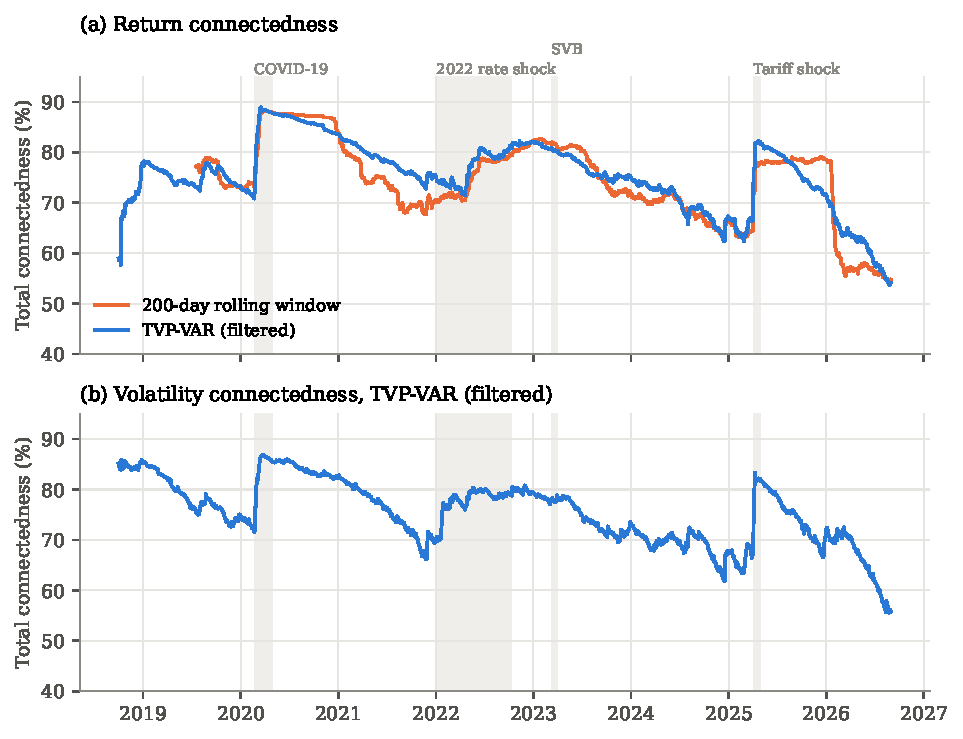
\includegraphics[width=\textwidth]{fig/fig1_tci.pdf}
\caption{Total connectedness index, daily. Panel (a): returns, filtered TVP-VAR and a 200-day rolling VAR. Panel (b): log range volatility, filtered TVP-VAR. Shaded: COVID-19 crash, 2022 rate shock, March 2023 bank failures, April 2025 tariff shock.}
\label{fig:tci}
\end{figure}

Net positions are persistent for some sectors and not for others (Figure~\ref{fig:net}). Industrials is a net transmitter on every day of the sample and Materials on all but a handful; Energy and Utilities are net receivers on every day. Information Technology changes sign. Its annual average NET is $+11.4$ in 2019 and $-13.8$ in 2024, a year in which its top-three share exceeded 60\%. Consumer Staples moves from roughly zero to $-17.2$ in 2025 as its top-three share rises from 38\% to 49\%. Section~\ref{sec:conc} tests whether these movements are systematic.

\begin{figure}[H]
\centering
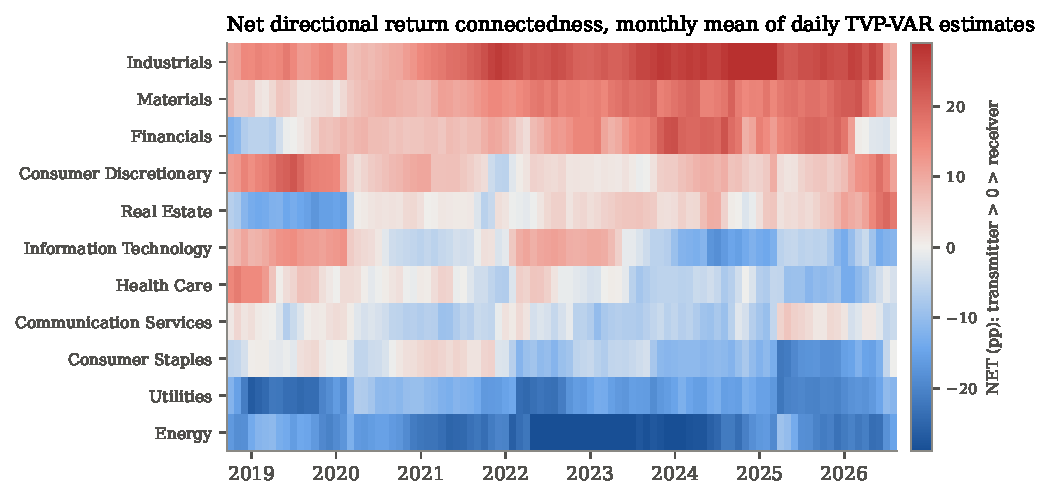
\includegraphics[width=\textwidth]{fig/fig2_net_heatmap.pdf}
\caption{Net directional return connectedness by sector, monthly average of daily filtered TVP-VAR estimates. Red: net transmitter. Blue: net receiver. Sectors ordered by full-sample mean.}
\label{fig:net}
\end{figure}

\subsection{Lead-lag relationships}\label{sec:granger}

Table~\ref{tab:granger} reports Granger tests across the 110 ordered pairs. Rows (1) to (4) use classical statistics. Taking the minimum $p$-value over lags one to five for each pair, a procedure that is common in applied work, gives 94 raw rejections and 90 after FDR control. Fixing the lag at five reduces this to 77, fixing it at one to 48, and conditioning on the full system to 20. Rows (5) to (7) use HC3 Wald statistics. No link survives FDR control, in the bivariate or system form, at lag one or five, in the full sample or either half.

\begin{table}[H]
\centering
\caption{Granger causality among 110 ordered sector pairs, daily returns}
\label{tab:granger}
\small
\begin{tabular}{llrrr}
\toprule
& Test & Raw $p<0.05$ & FDR & Bonferroni \\
\midrule
\multicolumn{5}{l}{\textit{Full sample, classical statistics}} \\
(1) & Bivariate F, minimum $p$ over lags 1 to 5 & 94 & 90 & \\
(2) & Bivariate F, lag 5 & 80 & 77 & \\
(3) & Bivariate F, lag 1 & 65 & 48 & \\
(4) & System VAR(1), Wald & 40 & 20 & \\
\multicolumn{5}{l}{\textit{Full sample, HC3 Wald}} \\
(5) & Bivariate, lag 1 & 20 & 0 & 0 \\
(6) & Bivariate, lag 5 & 20 & 0 & 0 \\
(7) & System VAR(1) & 6 & 0 & 0 \\
\multicolumn{5}{l}{\textit{Subsamples}} \\
(8) & System VAR(1), HC3, Oct 2018 to Aug 2022 & 15 & 0 & 0 \\
(9) & System VAR(1), HC3, Sep 2022 to Aug 2026 & 4 & 0 & 0 \\
(10) & As (1), excluding 20 Feb to 30 Jun 2020 & 22 & 0 & \\
(11) & As (1), 2021 to 2026 & 12 & 0 & \\
(12) & As (1), calendar 2020 only & 89 & 87 & \\
\bottomrule
\end{tabular}

\smallskip
\parbox{0.95\textwidth}{\footnotesize About 5.5 raw rejections are expected by chance at the 5\% level. FDR is \citet{benjamini1995} at 5\%.}
\end{table}

A Monte Carlo experiment explains the gap. We simulate returns from a one-factor model in which the factor and each sector's residual follow GARCH(1,1) processes with Student-$t$ innovations, all estimated on the fund returns, and in which no sector's lag predicts any other sector. The factor process is highly persistent ($\hat\alpha=0.159$, $\hat\beta=0.815$, $\hat\nu=7.1$). With 1,989 observations and 1,000 replications, the classical F-test at lag five rejects a true null 21.0\% of the time at a nominal 5\%, and the minimum-over-lags procedure rejects 30.7\% of the time. HC3 tests reject 5.2\% (lag one) and 4.1\% (lag five). Over 100 replications of the full 110-pair procedure, the classical minimum-over-lags approach produces 5.3 false FDR survivors on average, with 16.5 at the 90th percentile; HC3 produces 0.09.

The simulation produces far fewer false survivors than the 90 found in the data, so heteroskedasticity inflates the classical test but does not by itself account for the count. Rows (10) to (12) of Table~\ref{tab:granger} locate the rest. Excluding 20 February to 30 June 2020, 4.6\% of trading days, removes every classical FDR survivor, while calendar 2020 alone produces 87. That window contains 97.6\% of the lag-one cross-covariance between sectors over the whole sample. Inside it, the average lag-one correlation between one sector's return and another's is $-0.29$, almost equal to the average own-lag correlation of $-0.28$. Each sector's lagged return predicts the others only because all sectors reversed together from one day to the next. It is a market-wide reversal during the crash, not transmission from one sector to another, and even within the window no link survives HC3 testing with FDR control.

Out of sample, the lagged returns of other sectors carry no usable information (Table~\ref{tab:oos}). $R^2_{OS}$ is negative for all eleven sectors, between $-4.0\%$ and $-8.8\%$ for the unrestricted regression and between $-0.1\%$ and $-1.9\%$ for the combination forecast. One of 22 Clark-West tests rejects at 5\% and none after FDR control.

\begin{table}[H]
\centering
\caption{Out-of-sample predictability of next-day sector returns, 23 September 2020 to 31 August 2026}
\label{tab:oos}
\small
\begin{tabular}{lrrrr}
\toprule
& \multicolumn{2}{c}{All 11 lagged returns} & \multicolumn{2}{c}{Combination of 11 forecasts} \\
\cmidrule(lr){2-3}\cmidrule(lr){4-5}
Sector & $R^2_{OS}$ (\%) & CW $p$ & $R^2_{OS}$ (\%) & CW $p$ \\
\midrule
Communication Services & $-5.63$ & 0.42 & $-0.95$ & 0.33 \\
Consumer Discretionary & $-5.23$ & 0.55 & $-0.59$ & 0.37 \\
Consumer Staples & $-5.78$ & 0.60 & $-1.87$ & 0.76 \\
Energy & $-4.02$ & 0.03 & $-0.14$ & 0.21 \\
Financials & $-8.83$ & 0.13 & $-1.65$ & 0.65 \\
Health Care & $-7.53$ & 0.47 & $-1.48$ & 0.79 \\
Industrials & $-8.09$ & 0.45 & $-0.81$ & 0.44 \\
Information Technology & $-4.99$ & 0.23 & $-0.72$ & 0.11 \\
Materials & $-6.19$ & 0.32 & $-0.75$ & 0.42 \\
Real Estate & $-6.97$ & 0.44 & $-1.38$ & 0.73 \\
Utilities & $-7.79$ & 0.93 & $-1.19$ & 0.71 \\
\bottomrule
\end{tabular}

\smallskip
\parbox{0.95\textwidth}{\footnotesize Expanding-window OLS; benchmark is the prevailing mean. CW is the one-sided \citet{clark2007} test.}
\end{table}

These results bear on how connectedness should be read. The directional measures in Table~\ref{tab:static} describe how contemporaneous shocks are shared, identified through the generalized decomposition. They do not describe one sector's returns forecasting another's, and they should not be used to motivate daily sector-rotation rules.

\subsection{Concentration and connectedness}\label{sec:conc}

Table~\ref{tab:panel} reports regression (3). With sector and month fixed effects, a higher lagged top-three share lowers a sector's TO and NET connectedness in both systems. For returns, one percentage point of top-three share lowers NET by 0.47 points ($t=-3.6$) and TO by 0.50 points ($t=-2.5$). For volatility the coefficients are $-0.40$ for both ($t=-2.3$ and $-2.1$). The effect on FROM is zero in both systems. Concentrated sectors send fewer shocks; they do not receive fewer. The HHI coefficients have the same sign and are smaller relative to their standard errors (NET $-0.34$, $t=-1.7$).

\begin{table}[H]
\centering
\caption{Within-sector concentration and connectedness: two-way fixed effects}
\label{tab:panel}
\small
\begin{tabular}{lrrrrrr}
\toprule
& \multicolumn{3}{c}{Returns} & \multicolumn{3}{c}{Log range volatility} \\
\cmidrule(lr){2-4}\cmidrule(lr){5-7}
& FROM & TO & NET & FROM & TO & NET \\
\midrule
\multicolumn{7}{l}{\textit{Panel A: top-three share}} \\
Top-3 share$_{m-1}$ & $-0.037$ & $-0.502$ & $-0.465$ & $0.001$ & $-0.397$ & $-0.398$ \\
& (0.080) & (0.203) & (0.130) & (0.041) & (0.190) & (0.171) \\
$\ln$ index share$_{m-1}$ & $-7.42$ & $-16.61$ & $-9.19$ & $-1.16$ & $-0.90$ & $0.27$ \\
& (1.91) & (4.44) & (2.72) & (1.89) & (4.76) & (3.68) \\
Own log volatility & $-2.27$ & $-14.95$ & $-12.68$ & $-3.25$ & $-15.97$ & $-12.72$ \\
& (1.70) & (3.57) & (2.12) & (1.23) & (5.03) & (5.04) \\
Within $R^2$ & 0.047 & 0.118 & 0.167 & 0.015 & 0.058 & 0.054 \\
\midrule
\multicolumn{7}{l}{\textit{Panel B: Herfindahl index (controls as in Panel A)}} \\
HHI$_{m-1}$ & $0.008$ & $-0.335$ & $-0.342$ & $0.009$ & $-0.250$ & $-0.259$ \\
& (0.119) & (0.316) & (0.201) & (0.062) & (0.372) & (0.347) \\
\bottomrule
\end{tabular}

\smallskip
\parbox{0.95\textwidth}{\footnotesize 11 sectors, 94 months, 1,034 observations. Dependent variables are monthly means of daily filtered TVP-VAR measures from fund returns, in percentage points. Concentration in percentage points. Sector and month fixed effects. Driscoll-Kraay standard errors (three lags) in parentheses.}
\end{table}

Fund weight caps are a natural concern. They cut the weights of the largest names in precisely the most concentrated sectors, so the fund return understates the concentration we measure. Table~\ref{tab:robust} addresses this in two ways. When connectedness is re-estimated on the uncapped constituent returns, so that returns and concentration share one set of weights, every coefficient grows: NET falls by 0.66 points per point of top-three share ($t=-4.8$), TO by 0.83 ($t=-3.9$), and the HHI coefficients become significant (NET $-0.70$, $t=-2.6$; TO $-0.92$, $t=-2.3$). A small negative effect on FROM appears for the top-three share ($-0.17$, $t=-2.2$). Dropping Information Technology and Communication Services, the sectors where caps bind hardest, leaves the results intact on both return series.

\begin{table}[H]
\centering
\caption{Robustness of the concentration effect}
\label{tab:robust}
\small
\begin{tabular}{llrrr}
\toprule
Returns & Concentration & FROM & TO & NET \\
\midrule
Funds (baseline) & Top-3 & $-0.04$ (0.08) & $-0.50$ (0.20) & $-0.47$ (0.13) \\
& HHI & $0.01$ (0.12) & $-0.34$ (0.32) & $-0.34$ (0.20) \\
Constituents, uncapped & Top-3 & $-0.17$ (0.08) & $-0.83$ (0.21) & $-0.66$ (0.14) \\
& HHI & $-0.23$ (0.14) & $-0.92$ (0.40) & $-0.70$ (0.27) \\
Funds, excl. IT and COM & Top-3 & $-0.05$ (0.11) & $-0.60$ (0.23) & $-0.56$ (0.14) \\
& HHI & $-0.12$ (0.22) & $-0.87$ (0.54) & $-0.76$ (0.36) \\
Constituents, excl. IT and COM & Top-3 & $-0.11$ (0.09) & $-0.70$ (0.21) & $-0.58$ (0.13) \\
& HHI & $-0.27$ (0.19) & $-1.21$ (0.52) & $-0.94$ (0.35) \\
\bottomrule
\end{tabular}

\smallskip
\parbox{0.95\textwidth}{\footnotesize Return connectedness. Specification as in Table~\ref{tab:panel}; coefficient on lagged concentration with Driscoll-Kraay standard errors.}
\end{table}

Figure~\ref{fig:link} shows both sources of variation. Panel (a) is the cross-section of sector means, which the fixed effects remove: Industrials, the least concentrated sector, is the largest transmitter, and the correlation between mean top-three share and mean NET across the eleven sectors is $-0.40$. Panel (b) is the within-sector relationship behind Table~\ref{tab:panel}, after removing fixed effects and controls. It is monotone across the bins rather than driven by a few extreme observations.

\begin{figure}[H]
\centering
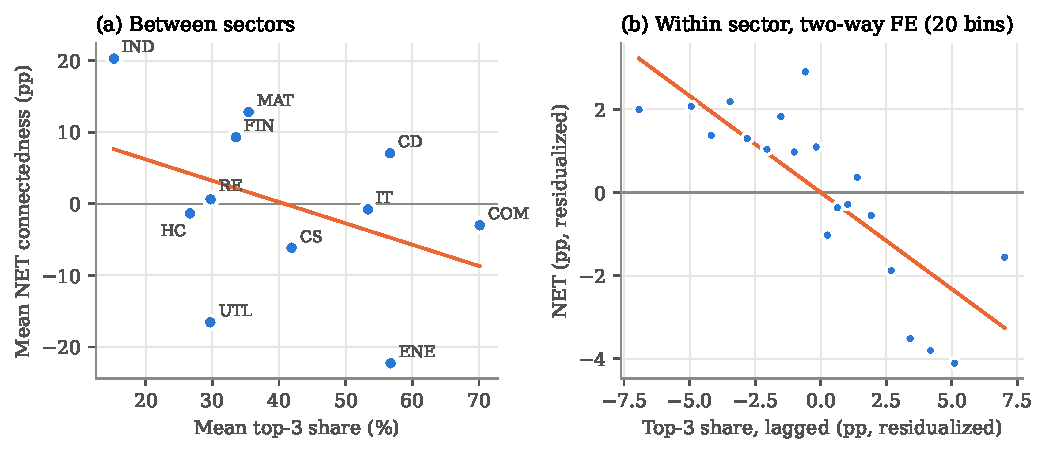
\includegraphics[width=\textwidth]{fig/fig4_concentration_link.pdf}
\caption{Top-three share and net return connectedness. Panel (a): sector means over the sample. Panel (b): binned scatter of lagged top-three share and NET after removing sector and month fixed effects, log index share, and own volatility; 20 equal-count bins; line is the OLS fit on all observations.}
\label{fig:link}
\end{figure}

The effect is a level effect. In first differences with month effects removed, the coefficients are small and insignificant (returns, NET: $-0.09$, $t=-0.8$). Concentration moves slowly, and month-to-month changes are dominated by price noise in a handful of stocks, so a first-difference test has little power against a relationship that operates through the level of a sector's composition.

\textbf{Mechanism.} The granular view predicts that a concentrated sector's return carries more firm-specific news and therefore co-moves less with the market. We test this with the monthly $R^2$ of each sector's daily return on the equal-weighted return of the other ten sectors, regressed on lagged concentration with the controls and fixed effects of regression (3). The average $R^2$ is 47\%. A one-point increase in top-three share lowers it by 0.56 points on fund returns ($t=-3.3$) and by 0.75 points on constituent returns ($t=-4.6$); the HHI coefficient is $-0.89$ ($t=-2.7$) on constituent returns. Concentrated sectors are less tied to the rest of the market, which is why their shocks explain less of other sectors' variance.

\textbf{Index level.} The same pattern appears in aggregate. Monthly total return connectedness is negatively related to the index top-ten share after controlling for log VIX (coefficient $-0.54$ per point, Newey-West $t=-2.1$, $R^2=0.38$), and more strongly for volatility connectedness ($-0.75$, $t=-4.3$). Both series trend over the sample, and neither relationship survives in first differences ($t=1.2$ and $0.7$), so the index-level result is descriptive. The sector panel, which removes common time variation with month fixed effects, carries the identification.

%============================================================
\section{Discussion}\label{sec:disc}
%============================================================

Concentration has two effects that are easy to confuse. At the index level, a few firms carry a large share of the market's risk, and a shock to one of them moves the index. At the sector level, the same firms make their own sectors' returns more idiosyncratic relative to other sectors. The first effect raises the importance of single names for index investors. The second lowers the importance of those sectors as channels for shocks between sectors. The evidence here is on the second effect: as a sector concentrates, it becomes less of a transmitter and less correlated with the rest of the market. This is consistent with the observation that total connectedness reached its sample low in 2026 at a time of record index concentration, although the time-series evidence alone cannot separate concentration from other trends.

For risk management the implication is that sector labels become less informative about common exposure as sectors concentrate. A sector whose top three firms hold four-fifths of its value behaves more like a basket of three stocks than like a diversified slice of the economy. Diversification measured across sectors can therefore look better than diversification measured across the firms that actually carry the weight.

The Granger results carry a separate lesson. Daily sector returns are close to unpredictable from each other's lags. Apparent evidence to the contrary comes from classical tests applied to heteroskedastic data and from a single crisis window, and it disappears under inference that allows for heteroskedasticity. The connectedness measures remain informative, but as measures of contemporaneous shock sharing.

Two limitations matter most. First, the constituent panel covers 85\% of index members at the start of the sample, because firms acquired and delisted before 2026 cannot be recovered; the missing firms are mostly small, and their absence overstates early concentration, which biases the time trend in concentration toward zero rather than away from it. Second, the evidence is an association in levels over eight years. It holds across return series, concentration measures, fund weight caps, and controls for size and volatility, but it is not a causal estimate, and a sector's composition and its connectedness could both respond to a third factor that moves slowly within sectors.

%============================================================
\section{Conclusion}
%============================================================

Sectors of the S\&P 500 share shocks within the day but do not forecast each other from one day to the next. Their connectedness peaked in the COVID-19 crash and reached its lowest level of the sample in August 2026. Within sectors, higher concentration goes with transmitting less: a sector dominated by a few firms carries more firm-specific news, co-moves less with the rest of the market, and explains less of other sectors' forecast-error variance. As index concentration continues to rise, sector-level measures of systemic linkage should be read together with the concentration of the sectors themselves. A frequency decomposition of the concentration effect, and a firm-level version that measures how much of each sector's transmission runs through its largest names, are natural next steps.

\bigskip
\noindent\textbf{Data availability.} Fund prices, index constituents and share counts are from public sources: Yahoo Finance for prices, share counts and the VIX; Wikipedia's list of S\&P 500 companies for current GICS classifications and addition dates; and a publicly maintained file of historical S\&P 500 membership for removals. The processed data and code that reproduce every table and figure are available from the author on request.

%============================================================
\begin{thebibliography}{99}
\setlength{\itemsep}{2pt}

\bibitem[Antonakakis et~al.(2020)]{antonakakis2020}
Antonakakis, N., Chatziantoniou, I., and Gabauer, D. (2020). Refined measures of dynamic connectedness based on time-varying parameter vector autoregressions. \textit{Journal of Risk and Financial Management}, 13(4), 84.

\bibitem[Barun\'ik and K\v{r}ehl\'ik(2018)]{barunik2018}
Barun\'ik, J., and K\v{r}ehl\'ik, T. (2018). Measuring the frequency dynamics of financial connectedness and systemic risk. \textit{Journal of Financial Econometrics}, 16(2), 271-296.

\bibitem[Benjamini and Hochberg(1995)]{benjamini1995}
Benjamini, Y., and Hochberg, Y. (1995). Controlling the false discovery rate: A practical and powerful approach to multiple testing. \textit{Journal of the Royal Statistical Society: Series B}, 57(1), 289-300.

\bibitem[Billio et~al.(2012)]{billio2012}
Billio, M., Getmansky, M., Lo, A. W., and Pelizzon, L. (2012). Econometric measures of connectedness and systemic risk in the finance and insurance sectors. \textit{Journal of Financial Economics}, 104(3), 535-559.

\bibitem[Campbell et~al.(2001)]{campbell2001}
Campbell, J. Y., Lettau, M., Malkiel, B. G., and Xu, Y. (2001). Have individual stocks become more volatile? An empirical exploration of idiosyncratic risk. \textit{Journal of Finance}, 56(1), 1-43.

\bibitem[Campbell and Thompson(2008)]{campbell2008}
Campbell, J. Y., and Thompson, S. B. (2008). Predicting excess stock returns out of sample: Can anything beat the historical average? \textit{Review of Financial Studies}, 21(4), 1509-1531.

\bibitem[Clark and West(2007)]{clark2007}
Clark, T. E., and West, K. D. (2007). Approximately normal tests for equal predictive accuracy in nested models. \textit{Journal of Econometrics}, 138(1), 291-311.

\bibitem[Diebold and Yilmaz(2009)]{diebold2009}
Diebold, F. X., and Yilmaz, K. (2009). Measuring financial asset return and volatility spillovers, with application to global equity markets. \textit{Economic Journal}, 119(534), 158-171.

\bibitem[Diebold and Yilmaz(2012)]{diebold2012}
Diebold, F. X., and Yilmaz, K. (2012). Better to give than to receive: Predictive directional measurement of volatility spillovers. \textit{International Journal of Forecasting}, 28(1), 57-66.

\bibitem[Diebold and Yilmaz(2014)]{diebold2014}
Diebold, F. X., and Yilmaz, K. (2014). On the network topology of variance decompositions: Measuring the connectedness of financial firms. \textit{Journal of Econometrics}, 182(1), 119-134.

\bibitem[Driscoll and Kraay(1998)]{driscoll1998}
Driscoll, J. C., and Kraay, A. C. (1998). Consistent covariance matrix estimation with spatially dependent panel data. \textit{Review of Economics and Statistics}, 80(4), 549-560.

\bibitem[Gabaix(2011)]{gabaix2011}
Gabaix, X. (2011). The granular origins of aggregate fluctuations. \textit{Econometrica}, 79(3), 733-772.

\bibitem[Grullon et~al.(2019)]{grullon2019}
Grullon, G., Larkin, Y., and Michaely, R. (2019). Are US industries becoming more concentrated? \textit{Review of Finance}, 23(4), 697-743.

\bibitem[Hong et~al.(2007)]{hong2007}
Hong, H., Torous, W., and Valkanov, R. (2007). Do industries lead stock markets? \textit{Journal of Financial Economics}, 83(2), 367-396.

\bibitem[Hou(2007)]{hou2007}
Hou, K. (2007). Industry information diffusion and the lead-lag effect in stock returns. \textit{Review of Financial Studies}, 20(4), 1113-1138.

\bibitem[Koop et~al.(1996)]{koop1996}
Koop, G., Pesaran, M. H., and Potter, S. M. (1996). Impulse response analysis in nonlinear multivariate models. \textit{Journal of Econometrics}, 74(1), 119-147.

\bibitem[Koop and Korobilis(2013)]{koop2013}
Koop, G., and Korobilis, D. (2013). Large time-varying parameter VARs. \textit{Journal of Econometrics}, 177(2), 185-198.

\bibitem[Menzly and Ozbas(2010)]{menzly2010}
Menzly, L., and Ozbas, O. (2010). Market segmentation and cross-predictability of returns. \textit{Journal of Finance}, 65(4), 1555-1580.

\bibitem[Parkinson(1980)]{parkinson1980}
Parkinson, M. (1980). The extreme value method for estimating the variance of the rate of return. \textit{Journal of Business}, 53(1), 61-65.

\bibitem[Pesaran and Shin(1998)]{pesaran1998}
Pesaran, M. H., and Shin, Y. (1998). Generalized impulse response analysis in linear multivariate models. \textit{Economics Letters}, 58(1), 17-29.

\bibitem[Pollet and Wilson(2010)]{pollet2010}
Pollet, J. M., and Wilson, M. (2010). Average correlation and stock market returns. \textit{Journal of Financial Economics}, 96(3), 364-380.

\bibitem[Rapach et~al.(2019)]{rapach2019}
Rapach, D. E., Strauss, J. K., Tu, J., and Zhou, G. (2019). Industry return predictability: A machine learning approach. \textit{Journal of Financial Data Science}, 1(3), 9-28.

\end{thebibliography}

\end{document}
